\chapter{Introduction}
\label{chapter1}



This chapter introduces the related literature review, motivation and goals of the undertaken research.
The chapter begins with a brief preface of cryptology and its importance in the era Internet of Things (IoT) and Big Data.
In \secref{ch1_subsec_pkc} we present how Public-Key Cryptography (PKC) is shaping the security of our every day life.
We introduce the importance of Pairing-Based Cryptography(PBC) in \secref{ch1_subsec_pbc} for the next generation of security protocols. 
\secref{ch1_sec_motivation} presents the motivation behind the works undertaken to assemble of this thesis.
\secref{ch1_sec_outline} outlines the overall organization of this thesis.

\section{Cryptology}
\label{ch1_sec_crypto}
Cryptography is the science of communicating with the authentic receiver through an insecure channel in secret. 
Cryptanalysis is the techniques of breaking the secret communications.
Cryptology is the combination of these two domains.

The history of Cryptography dates back to the time of the Greek and Roman empire.
Julius Caesar used a simple shift and substitute system.
Up until the early '70s of the last century, cryptology was evolved mostly for military purposes. 
The cryptography got its first democratic form in 1975 when Diffie and Hellman invented the concept of public-key cryptography \cite{diffie1976new}. 
The concept was first realized by as practical cryptosystem by the works of Rivest, Shamir and Adleman (RSA) in 1977 \cite{rivest1978method}.
At the same time in 1977, National Bureau of Standards published a cryptosystem intended for the governmental agencies or banks with the named Data Encryption Standard (DES).
From then a new era of cryptography known as \textit{Modern cryptography} was initiated.
The well-organized procedures called \textit{protocols} is the basis of Modern cryptography.
One of the most elegant features of modern crypto-protocols is their inner algorithms are not secret yet withstand cryptanalysis from experts/attackers.
More importantly, these protocols are easy to use for people with no understanding of the underlying principles.
For example, paying by credit cards or withdrawing money using debit cards with a personal identification number (PIN) is doable without concerning what’s going on under the hood. 

The little basic functionality of modern cryptosystem is to enable a sender (Alice \footnote{Alice and Bob are fictional characters first used by Rivest, Shamir and Adleman in \cite{rivest1978method} as placeholder name in cryptology.}) to convert a message (plaintext) into a cipher (ciphertext) before sending to a legitimate receiver (Bob) over the public communication media. 
The receiver can convert the cipher back into the original message using secret information named as a key.
An adversary (Eve) eavesdrops in the middle of the conversation to retrieve information from the cipher.
The cipher is safe from to the adversary until the key is not compromised. 

Cryptography became more important as individuals and business increasingly depend on the Internet as a channel for communication. Therefore, the following four properties are the basis of a cryptosystem.


\begin{itemize}
\item Data confidentiality:
This property ensures that confidential information such as bank transactions or medical data etc. are secret from unauthorized entities. 

\item Data integrity:
When data is stored, this property ensures that it not only kept secret (Data confidentiality) but also not rigged.
Confidentiality and integrity is enforced by encryption.

\item Authentication:
In a connection-oriented communication authentication proves both parties identity before communication begins.
Digital signature is used for this purpose to sign a message electronically.
It shields the legitimate party against masquerader from impersonating as a trusted party.
This property gives the receiver a confidence to believe that the message sent over the insecure channel is indeed sent by the actual signee.

\item Non-repudiation:
Non-repudiation (with proof of origin and with proof of receipt) ensures that sender and receiver can not deny having taken part in a communication.
This is important for many cases especially e-commerce while communicating over the Internet.
\end{itemize}

The modern crypto-protocols fall in following two major categories. 

\subsection{Symmetric/Private-Key Cryptography}
Private-Key Cryptography, also known Symmetric Cryptography is the technique where both the sender and the receiver use same \textit{key} or easily derivable from one another to encrypt and decrypt a message.
This type of cryptography is very old history. 

Modern cryptosystems offer efficient symmetric cryptography algorithms, e.g Advanced Encryption Standard (AES) \cite{AES_DaemenR02}.
Such cryptography has two main obstacles i.e. \textit{Key management} and \textit{key establishment}.
Since the keys are same, they need to kept private (\textit{Key management})  in both ends and should be shared securely beforehand (\textit{Key establishment}) without physically meeting.

The Public-key Cryptography offers the solution for \textit{Key establishment} applying Diffie-Hellman key exchange.
This work primarily focuses on a certain type of Public-key Cryptography. 
The subsequent chapters will describe in details.

\subsection{Public-key Cryptography}
\label{ch1_subsec_pkc}
As afore mentioned, In 1976, Whitfield Diffie and Martin Hellman published their monumental work as a key exchange protocol. 

In the mid 80's the independent work of Miller \cite{C:Miller85} and Koblitz \cite{koblitz1987elliptic} began the journey of elliptic curve cryptosystems (ECC). 
The shorter key length for same security level than RSA, ECC became popular among the researchers. 

The problems of key distribution and storage associated with symmetric cryptography were the motivation behind the concept of Asymmetric Cryptography, also referred to as Public- Key Cryptography. The first practical public key protocol was introduced by Whitfield Diffie and Martin Hellman in 1976 [24] in the form of a key exchange protocol. The focus of this thesis is an area of asymmetric cryptography. The idea is to use keys kE and kD such that it is infeasible to calculate the one from the other. This way kE , referred to as the public key, can be published and anyone wishing to communicate with Alice, for example, just needs to find Alice’s public key from a list and encrypt the message; only Alice will be 

  \begin{figure}
    \centering
    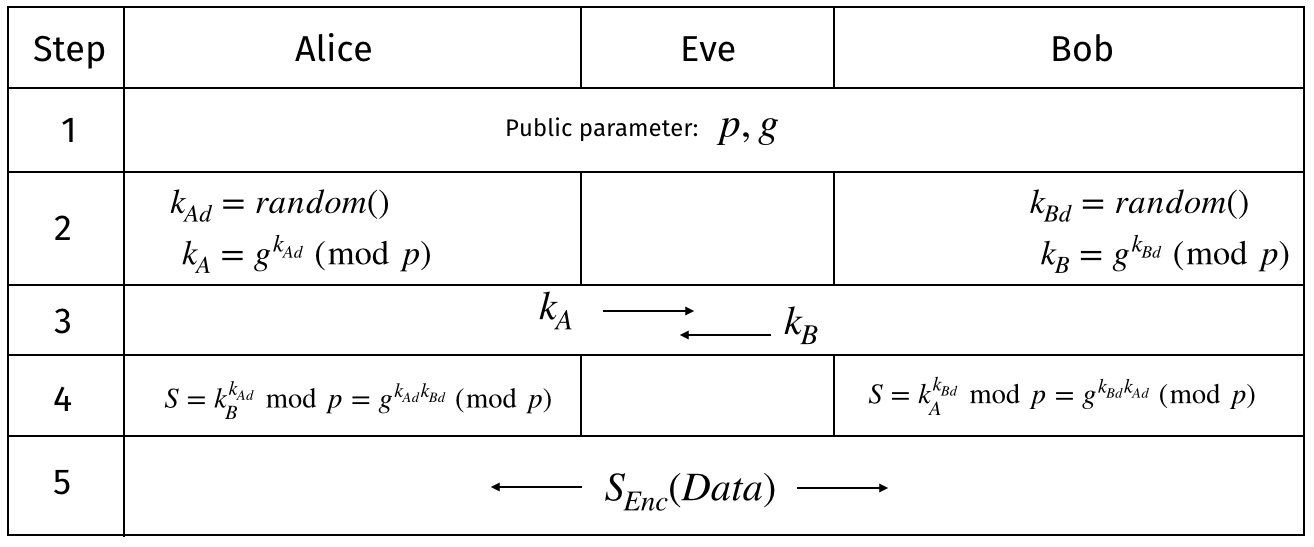
\includegraphics[width=.9\linewidth, height=.67\textheight, keepaspectratio]{Figures/DHKE}
    \caption{Exchanging shared secret key using DH-key exchange.}
  \end{figure}

able to decrypt the message using her corresponding private key. This concept solves the problem of securely distributing keys. What’s more, in a network of t people, only t keys are needed, a huge improvement on the situation using symmetric cryptography.
Asymmetric cryptography uses so called one-way mathematical problems; one-way problems consist of an operation which is easy to compute, but difficult to invert. Using one-way problems we are able to find key pairs kE and kD with the desired properties.
One such problem is the Integer Factoring Problem (IFP): given two large primes p and q, it is easy to multiply them together to find $l = pq$, but given an integer l, the product of two large primes, it is a much more difficult task to factor l to recover p and q.

\subsection{Pairing-Based Cryptography}
\label{ch1_subsec_pbc}
Human civilization is moving to a direction where data generated from the devices used in our daily life will define how smart our society will be.
In technical jargon we define that IoT (Internet of Things) era controlled by Data Science.
Some data can be mundane with no purpose and some data can be extraordinary important.
Let us imagine a case where the adversary takes controls heart beat monitor sensor of our smart watch or control sensors of self-driving car.
The outcome of the damage is unimaginable. 
There is not alternative to protect these data from unwanted access.
The challenge is, most of the IoT devices are computationally resource constrained.
In some devices it is somewhat impractical to generate key pairs for widely practiced security protocols.
There are several innovative solutions e.g. Broadcast encryption, or Identity based encryption that can solve such problems.
The above mentioned applications stands on a compelling topic of mathematics name pairing over elliptic curve.

\section{Motivation}
\label{ch1_sec_motivation}

\section{Our Contribution}
\label{ch1_sec_contribution}


\section{Thesis Outline}
\label{ch1_sec_outline}

With  the development of the information and communication technology, a social utilization of a computer network has advanced at a rapid pace.
As a result, several services associated with the society and our daily life such as e-commerce and e-government are provided on the computer network.
These services, however, transmit highly-confidential informations such as financial or privacy informations via the network.
In order to protect these informations, cryptosystems are indispensable that provides the secret communication and authentication for the current information and communication services.
%Cryptosystems are roughly classified into two types, 
In the modern cryptographies, public key cryptography that provides authentication, data integrity, and non-repudiation is one of the most important cryptosystems.

Recently, new cryptographic schemes that relax the restriction on use of the modern public key cryptosystems are proposed.
Among these innovative cryptographies, pairing-based cryptographies such as ID-based cryptographies \cite{ID} and group signature authentications \cite{BBS}, \cite{nakanisi} have received much attentions.
For example, in ID-based cryptographies, some unique information about the identity of the user such as e-mail address, name and telephone number can be used as the public key of user.
In addition, group signature authentications allow the service vendor to verify that a signature is signed by a valid user, but they can not know who is the signer.
Therefore, group signatures can protect user's privacy while preventing illegal accesses.

These cryptographic schemes allow us to use the advanced cryptosystems that can not be constructed by the conventional cryptographic technologies.
However, they have a problem with processing time because a fairly complex calculation is required for their processing.  
Due to this problem, these sophisticated cryptographies have not yet led to practical use.   
In order to make these cryptographic applications practical, this thesis proposes efficient methods to calculate operations required for pairing-based cryptographies.

%���@�\�ȈÍ����K�v
%%%%%%%%%%%%%%%%%%%%%%%%%%%%%
\section{Motivation}
%%%%%%%%%%%%%%%%%%%%%%%%%%%%%
Pairing is a bilinear map from two groups $\mathbb{G}_1$ and $\mathbb{G}_2$ to a group $\mathbb{G}_3$, where they have respectively same prime order $r$.
In detail, $\mathbb{G}_1$ and $\mathbb{G}_2$ respectively becomes a subgroup in an elliptic curve group $E(\F{q}{})$ and $E(\F{q}{k})$, and $\mathbb{G}_3$ becomes a subgroup in $\F{q}{k}$, where $q$ is a power of $p$ and an extension degree $k$ is especially called the {\it embedding degree}.
 
In pairing-based cryptography, not only pairing calculation but also scalar multiplications in $\mathbb{G}_1$ and $\mathbb{G}_2$, and exponentiations in $\mathbb{G}_3$ are carried out.
Among these operations, since pairing is the highest cost operation, a lot of improvements for pairing such as $\eta_T$ pairing over super singular curves and Ate \cite{Hess}, {\it twisted} Ate\cite{Hess}, {\it optimized} Ate \cite{TAte}, optimized {\it twisted} Ate\cite{TAte}, $R$-ate\cite{Rate}, {\it Optimal}\cite{OptAte}, Xate \cite{Xate} pairings over ordinary curves, have been proposed in the recent years.
Among these pairings, the fastest pairing is $\eta_T$ pairing.
However, $\eta_T$ pairing has a disadvantage that supersingular curves are restricted to {\it embedding degree} $k\leq6$. 
Since the {\it embedding degree} is important parameter that determines the security level of pairing-based cryptographies, efficient pairings on ordinary curves whose {\it embedding degree} are flexibly selectable are required.
This thesis targets Ate and {\it twisted} Ate pairings because they are efficiently calculated on ordinary curves.
  
On the other hand, in addition to pairing, pairing-based cryptographies need to carry out a lot of scalar multiplications in $\mathbb{G}_1$ and $\mathbb{G}_2$ in proportion to the number of users.
Therefore, efficient scalar multiplications in $\mathbb{G}_1$ and $\mathbb{G}_2$ can reduce the total cost of pairing-based cryptography.

In this thesis, we propose efficient scalar multiplications in $\mathbb{G}_1$ and $\mathbb{G}_2$, and pairings based on Ate and {\it twisted} Ate pairings.

%scalar multiplication 
Let $P$ be a rational point in an elliptic curve group, a scalar multiplication $[s]P$ by scalar $s\in{\mathbb Z}$ means $(s-1)$-times elliptic curve additions of $P$.
General approach to accelerate a scalar multiplication is a binary method.
Note that a scalar $s$ is at most the order $r$.
Using a binary method, we can calculate $[s]P$ by $\lfloor \log_2 s \rfloor$-times elliptic curve doublings and Hw($s$)-times elliptic curve additions, where Hw($s$) means the number of 1s' in the binary representation of $s$ and it is generally called a {\it hamming weight} of $s$.  

To accelerate a scalar multiplication, it is important that the scalar multiplication of an intrinsic scalar $\lambda$ is calculated by efficiently computable endomorphisms.
If the scalar $\lambda$ is smaller than the order of an elliptic curve group, we can decompose a target scalar by $\lambda$-adic expansion.
By using multi-scalar multiplication techniques, we can reduce the number of elliptic curve doublings to the bit-size of the scalar $\lambda$ corresponding to the endomorphism.
For example, when the elliptic curve is defined over an extension field, Frobenius endomorphism $\phi$ will efficiently work.
Note that a Frobenius endomorphism is free from arithmetic operations.
In the case of $\mathbb{G}_2$ of Ate and {\it twisted} Ate pairings, let $t$ be a Frobenius trace of elliptic curve, a scalar multiplication by $\lambda = (t-1)$ corresponds to $\phi(P)$.
Since $t\approx\sqrt{r}$ from Hasse's theorem, the number of elliptic doublings are reduced by about half.
This relation $\phi(P)=[t-1]P$ has been considered optimal because the trace is the smallest among parameters construct an elliptic curve. 

%�Ȑ��̘b
On the other hand, recent elliptic curves for pairing need one more parameter in addition to parameters such as $p$, $t$, and $r$.  
Elliptic curves over which pairing can be defined are called pairing-friendly curves.
In general, it is difficult to generate such pairing-friendly curves because they need to satisfy some strict conditions.
However, several methods to easily generate pairing-friendly curves are proposed in recent years \cite{Taxo}.
For example, {\it families} of pairing friendly curves whose parameters such as characteristic $p$, order $r$, and trace $t$ are given by polynomials in terms of integer $\chi$ are easily constructed.
Especially, since {\it complete families} can generate a lot of elliptic curves, we can select the optimal curve suitable for pairing calculations and scalar multiplications.
Among {\it families} of pairing friendly curves, there is a curve whose trace $t$ is given by polynomial that has larger degree than or equal to 2.
In this case, $\chi$ becomes the smallest among parameters to construct curves.
Therefore, it is possible that we can obtain the relation that joins Frobenius maps and an intrinsic scalar that is smaller than trace $t$.
Thus, it is important to optimize the relation available for a scalar multiplication for {\it families} of pairing friendly curves.
This thesis targets {\it families} of pairing-friendly curves, and we mainly deal with Barreto-Naehrig (BN) curves of {\it embedding degree} equal to 12 that is one of the most important {\it complete families} of pairing-friendly curves.

%G2�̘b
In the case of BN curves, we can obtain the key relation that joins Frobenius maps and a certain smaller scalar than $t$.
In detail, since the scalar becomes about $\chi$ and $t$ is given by $(6\chi^2+1)$, its bit-size becomes a half of $t$.
 
%G1�̘b
In the case of $\mathbb{G}_2$, Frobenius endomorphism efficiently works for a scalar multiplication.
However, Frobenius endomorphism does not work for a rational point $\mathbb{G}_1$ because a rational point applied Frobenius map becomes itself.
Therefore, an efficiently computable endomorphism in $\mathbb{G}_1$ is required to apply the technique with Frobenius map as a scalar multiplication in $\mathbb{G}_2$.
This thesis proposes a Frobenius-like endomorphism on $\mathbb{G}_1$.
Using twist techniques, we can prepare the another group that is isomorphic to $\mathbb{G}_1$ over an extension field. 
Therefore, let the group be $\mathbb{G}_1'$, we can use Frobenius endomorphism on $\mathbb{G}_1'$.
Focusing on this property, we derive a new endomorphism from the endomorphism on $\mathbb{G}_1'$.
Then, we optimize a key relation available for a scalar multiplication in $\mathbb{G}_1$ that joins a new endomorphism and a certain scalar.
  
Furthermore, we apply the key relations available for scalar multiplications in $\mathbb{G}_1$ and $\mathbb{G}_2$ to accelerating pairing calculations.

%pairing
The calculation costs of pairing are the highest among operations required for pairing-based cryptographies.
Since pairing calculation is inherently sequential, it is difficult to apply the efficient parallelization technique using some recent processors have several computation cores.
In general, pairing calculations consists of two calculation parts, one is Miller's algorithm and the other is {\it final exponentiation}.
Since Miller's algorithm is slower than {\it final exponentiation}, several improvements for Miller's algorithm such as Ate and {\it twisted} Ate have been proposed.
A structure of the algorithm is approximately same as that of a binary method for a scalar multiplication.
Therefore, Miller's algorithm iterates a certain process $\lfloor \log_2 s \rfloor$-times as a binary method, where $s$ is a parameter gives an loop iterations of Miller's algorithm.
Since the process in Miller's algorithm needs several operations such as elliptic curve additions in elliptic curves and multiplications in extension fields, pairing becomes a fairly complex operation. 
Though a scalar multiplication uses a random number $s$, the number of calculations of Miller's algorithm is given by a specific number.
For example, the number of calculation loops of Miller's algorithm for Ate pairing is given by $\lfloor \log_2 (t-1) \rfloor$.
That is, the calculation costs of Miller's algorithm is determined by the number of loop iterations.
Therefore, we can reduce the calculation costs of Miller's algorithm by reducing its number of iterations.
In addition, Hess shows that the lower bound of the number of iterations of Miller's algorithm for each pairing-friendly curve.
In the case of BN curves, it becomes about $\lfloor \log_2 \chi \rfloor$, however Ate and {\it twisted} Ate pairing does not achieve.
  
  %Xate
In the case of a scalar multiplication, we can reduce the number of elliptic curve doublings by decomposing a scalar with the key relation.
Using divisor theorem, a Miller's algorithm can be also decompose into several Miller's algorithm calculations whose the number of iterations are small.
However, since there is no efficiently computable Miller's algorithm calculation for a certain number of iterations, the decomposition does not work.  
Rather, when we decompose Miller's algorithm, extra operations such as exponentiations in extension fields are required.
This thesis shows that when we decompose a Miller's algorithm into several Miller's algorithms, some decomposed Miller's algorithms that has the bilinearity after applying {\it final exponentiation} can be skipped by using the property of bilinearity.
In the case of Ate pairing, Miller's algorithm has the bilinearity when a parameter that gives the number of iteration is equal to $(t-1)$.
Therefore, the key relation for a scalar multiplication in $\mathbb{G}_2$ is closely related to Ate pairing.
In this thesis, Miller's algorithm is decomposed using the key relation, and then a new pairing whose number of iterations for Miller's algorithm is smaller than that of Ate pairing is proposed.
As a result, the proposed pairing achieves the lower bound of the number of iterations for Miller's algorithm.
Meanwhile, focusing on the decomposition technique for Miller's algorithm, Vercauteren, Lee et al. and the authors have respectively proposed Optimal, $R$-ate, and Xate pairings, independently.
Optimal and $R$-ate pairings also achieve the lower bound of the number of iterations for Miller's algorithm.
This thesis compares these pairings with our proposed pairing (Xate pairing).

%twisted Xate �̘b
On the other hand, the number of iterations for {\it twisted} Ate pairing is closely related to the key relation for a scalar multiplication in $\mathbb{G}_1$.
That is, a new pairing based on {\it twisted} Ate pairing is derived, since its Miller's algorithm can be efficiently decomposed by the key relation. 
This pairing have been proposed by Lee et al. as {\it twisted} $R$-ate pairing, but the pairing does not achieve the lower bound of number of iterations for Miller's algorithm.
In detail, the number of iterations is twice larger than that of the proposed pairing based on Ate pairing in the case of BN curves.
This thesis first derives an another key relation that decomposes Miller's algorithm of {\it twisted} Ate pairing to two Miller's algorithm calculations whose maximum number of iterations is equal to that of the proposed pairing based on Ate pairing using the key relation available for a scalar multiplication in $\mathbb{G}_1$.
Then, using a precomputed scalar multiplication, we propose a method to parallelize the two Miller's algorithm calculations with multi-pairing or {\it thread-computing}. 

Since the proposed methods can substantially improve operations such as scalar multiplications and pairings required for pairing-based cryptographies, we can help to solve the problem on processing times.  
Therefore, our research contributes to promoting sophisticated cryptographies such as ID-based cryptographies and group signature authentications. 


%%%%%%%%%%%%%%%%%%%%%%%%%%%%%
\section{Outline}
%%%%%%%%%%%%%%%%%%%%%%%%%%%%%

This thesis is organized as follows: 

In Chapter 2, we briefly review the mathematical fact to define the pairing, and describe about the conventional pairing such as Tate, Ate, {\it twisted} Ate pairings.
In addition, a target class of elliptic curves are shown.
Ate and {\it twisted} Ate pairings improves Tate pairing by setting certain groups that have a special properties to $\mathbb{G}_1$ and $\mathbb{G}_2$.
In this thesis, we target Ate and {\it twisted} Ate pairings, and accelerates scalar multiplications in their $\mathbb{G}_1$ and $\mathbb{G}_2$.
In addition, new pairings respectively based on Ate and {\it twisted} Ate pairings are proposed.  
%
Chapter 3 proposes an efficient scalar multiplication in $\mathbb{G}_2$ that used by Ate and {\it twisted} Ate pairings.
To accelerate a scalar multiplication, it is important that a certain scalar multiplication is calculated by efficiently computable endomorphisms.
A target $\mathbb{G}_2$ has a property that a certain scalar multiplication is calculated by Frobenius endomorphism that is efficiently computable.
Focusing on this property, we derive a key relation available for a scalar multiplication in $\mathbb{G}_2$ from the structural properties of target elliptic curves.
Then, using the key relation, an efficient scalar multiplication is proposed.
In addition, we show that the proposed scalar multiplication is about 40\% faster than the conventional method from experimental results.   

Chapter 4 proposes an efficient scalar multiplication in $\mathbb{G}_1$ that used by Ate and {\it twisted} Ate pairings.
A target $\mathbb{G}_1$ does not have a property that Frobenius endomorphism is available for a scalar multiplication.
Therefore, it is difficult to apply the method proposed in chapter 3 to a scalar multiplication in $\mathbb{G}_1$.
In order to solve this problem, we propose a new endomorphism available for a scalar multiplication in $\mathbb{G}_1$.
Using the endomorphism, a key relation is derived in a same manner of $\mathbb{G}_2$.
Then, using the key relation, an efficient scalar multiplication is proposed.   
In addition, this chapter shows that the proposed method is about 30\% faster than the conventional method from experimental results.   

In chapter 5, how to decompose the Miller's algorithm calculation is described, and it is shown that the approach for accelerating scalar multiplications is also applied to pairing calculations.
Then, we proposes a new pairing based on Ate pairing using the key relation available for a scalar multiplication in $\mathbb{G}_2$.
This is because the property of $\mathbb{G}_2$ is closely related to Ate pairing.
In addition, we show that the proposed pairing is about two times faster than Ate pairings from experimental results.   

Chapter 6 proposes an efficient pairing based on {\it twisted} Ate pairing using the key relation proposed in chapter 4.
In addition, the pairing can be efficiently applied the parallelizing technique that can not be applied to the conventional pairings.
From the experimental results, we show that the proposed method can reduce the calculation times of {\it twisted} Ate pairing by up to about 70\%. 

Chapter 7 concludes this thesis.